% Generated by: TimedRegex, Version = 1.0.0.0
% Date 5/12/2024 10:20:04 PM
\usetikzlibrary {automata,positioning}
% "A[1;1]+'"
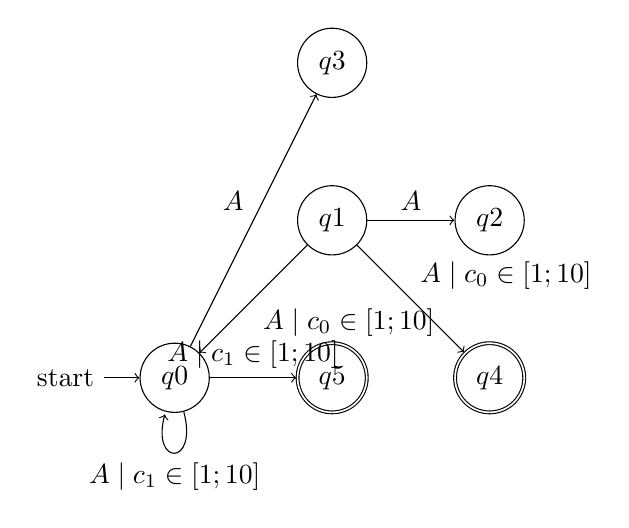
\begin{tikzpicture}[auto]
    \node[state, initial] at (0, 0)(q0){$q0$};
    \node[state] at (2, 2)(q1){$q1$};
    \node[state] at (4, 2)(q2){$q2$};
    \node[state] at (2, 4)(q3){$q3$};
    \node[state, accepting] at (4, 0)(q4){$q4$};
    \node[state, accepting] at (2, 0)(q5){$q5$};
    
    \path[->]
        (q1)edge node{$A$}(q2)
        (q0)edge node{$A$}(q3)
        (q1)edge node{$A\mid c_0\in[1;10]$}(q4)
        (q1)edge node{$A\mid c_0\in[1;10]$}(q0)
        (q0)edge node{$A\mid c_1\in[1;10]$}(q5)
        (q0)edge [loop below] node{$A\mid c_1\in[1;10]$}(q0)
        ;
    \label{fig:prune0}
\end{tikzpicture}
 
